\centering

\rotatebox{90}{
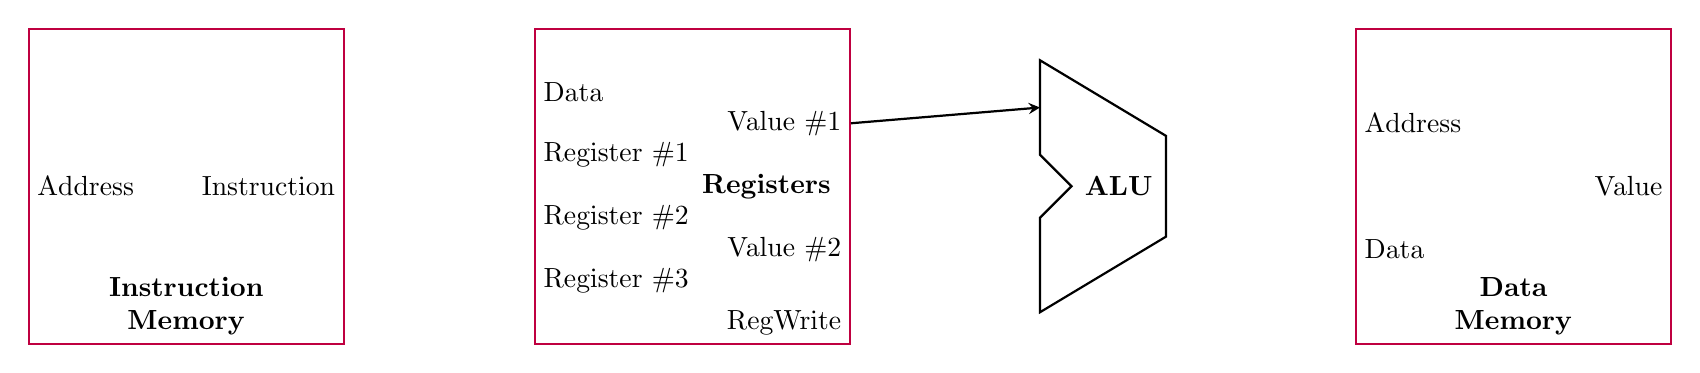
\begin{tikzpicture}[]
  \newcommand{\Xpc}[0]{ 0mm }
  \newcommand{\Xim}[0]{ 32mm }
  \newcommand{\Xreg}[0]{ 56mm }
  \newcommand{\Xloadmux}[0]{ 65mm }
  \newcommand{\Xdm}[0]{ 80mm }
  \newcommand{\Ycenter}[0]{ 8mm }
  
  \newcommand{\spacing}[0]{ 8mm }
  \newcommand{\lineheight}[0]{ 8mm }
  
  \tikzstyle{edge}  = [thick,>=stealth,draw=black]
  \tikzstyle{dedge} = [thick,->,>=stealth,draw=black]
  \tikzstyle{block}=[
    rectangle,
    draw=purple,
    anchor=center,
    align=center,
    thick,
  ]
  \tikzstyle{mux}=[
    rectangle,
    draw=purple,
    anchor=center,
    align=center,
    rounded corners=2mm,
    minimum width=4mm,
    thick,
  ]
  
  % #1: prefix
  % #2: position
  \newcommand{\buildInstructionMemoryBlock}[2]{
    \node[
      block,
      anchor=west,
      minimum width=40mm,
      minimum height=40mm,
    ] (#1) at (#2) {};
    \node[anchor=south,align=center] () at (#1.south) {\textbf{Instruction}\\\textbf{Memory}};
    
    \coordinate (#1 addr) at ([yshift=0.0*\lineheight]#1.west);
    \coordinate (#1 inst) at ([yshift=0.0*\lineheight]#1.east);
    
    \node[anchor=west] () at (#1 addr) {Address};
    \node[anchor=east] () at (#1 inst) {Instruction};
  }
  
  % #1: prefix
  % #2: position
  \newcommand{\buildRegisterBlock}[2]{
    \node[
      block,
      anchor=west,
      minimum width=40mm,
      minimum height=40mm,
    ] (#1) at (#2) {};
    \node[anchor=west] () at (#1.center) {\textbf{Registers}};
    
    \coordinate (#1 data)   at ([yshift= 1.5*\lineheight]#1.west);
    \coordinate (#1 regI)   at ([yshift= 0.5*\lineheight]#1.west);
    \coordinate (#1 regII)  at ([yshift=-0.5*\lineheight]#1.west);
    \coordinate (#1 regIII) at ([yshift=-1.5*\lineheight]#1.west);
    \coordinate (#1 valI)   at ([yshift= 1.0*\lineheight]#1.east);
    \coordinate (#1 valII)  at ([yshift=-1.0*\lineheight]#1.east);
    
    \node[anchor=west] () at (#1 data)   {Data};
    \node[anchor=west] () at (#1 regI)   {Register \#1};
    \node[anchor=west] () at (#1 regII)  {Register \#2};
    \node[anchor=west] () at (#1 regIII) {Register \#3};
    \node[anchor=east] () at (#1 valI)   {Value \#1};
    \node[anchor=east] () at (#1 valII)  {Value \#2};
    
    \node[anchor=south east] (#1 RegWrite) at (#1.south east) {RegWrite};
    \coordinate (#1 rw) at (#1 RegWrite.south);
  }
  
  % #1: prefix
  % #2: position
  \newcommand{\buildDataMemoryBlock}[2]{
    \node[
      block,
      anchor=west,
      minimum width=40mm,
      minimum height=40mm,
    ] (#1) at (#2) {};
    \node[anchor=south,align=center] () at (#1.south) {\textbf{Data}\\\textbf{Memory}};
    
    \coordinate (#1 addr)  at ([yshift= 1.0*\lineheight]#1.west);
    \coordinate (#1 data)  at ([yshift=-1.0*\lineheight]#1.west);
    \coordinate (#1 value) at ([yshift= 0.0*\lineheight]#1.east);
    
    \node[anchor=west] () at (#1 addr) {Address};
    \node[anchor=west] () at (#1 data) {Data};
    \node[anchor=east] () at (#1 value) {Value};
  }
  
  
  % #1: prefix
  % #2: position
  \newcommand{\buildALU}[3]{
    \newcommand{\aluheight}[0]{ 32mm }
    \newcommand{\aluwidth}[0]{ 16mm }
    \newcommand{\aluindent}[0]{ 4mm }
    
    \coordinate (offset) at (#2);
    
    \draw[
      thick,
    ]  ([yshift=\aluheight/2]offset)
    -- ([xshift=\aluwidth,yshift= \aluheight/5]offset)
    -- ([xshift=\aluwidth,yshift=-\aluheight/5]offset)
    -- ([yshift=-\aluheight/2]offset)
    -- ([yshift=-\aluindent]offset)
    -- ([xshift=\aluindent]offset)
    -- ([yshift=\aluindent]offset)
    -- cycle;
    \node[anchor=center,align=center] () at ([xshift=\aluindent+\aluwidth/2-\aluindent/2]offset) {\textbf{#3}};
    
    \coordinate (#1 iI)  at ([yshift= \aluheight/4+\aluindent/2]offset);
    \coordinate (#1 iII) at ([yshift=-\aluheight/4-\aluindent/2]offset);
    \coordinate (#1 o)   at ([xshift=\aluwidth]offset);
  }
  
  % program counter
%  \node[block] (pc) at (\Xpc, \Ycenter) {PC};
  
  % instruction increment alu
  
  % instruction branch alu
  
  % branch mux
  
  % instruction memory
  \coordinate (imcoord) at (\Xreg, \Ycenter);
  \buildInstructionMemoryBlock{im}{imcoord}
  
  % registers
  \buildRegisterBlock{reg}{[xshift=3*\spacing]im.east}
  
  % alu
  \buildALU{alu}{[xshift=3*\spacing] reg.east}{ALU}
  
  % data memory
  \buildDataMemoryBlock{dm}{[xshift=3*\spacing]alu o}
  
  % load mux
%  \node[mux] (loadmux) at ([yshift=12mm]$(reg)!0.5!(dm)$) {\rotatebox{90}{mux}};
  
  % wiring
  \draw[dedge] (reg valI) -- (alu iI);
\end{tikzpicture}
}
